% ****** Start of file aipsamp.tex ******
%
%   This file is part of the AIP files in the AIP distribution for REVTeX 4.
%   Version 4.1 of REVTeX, October 2009
%
%   Copyright (c) 2009 American Institute of Physics.
%
%   See the AIP README file for restrictions and more information.
%
% TeX'ing this file requires that you have AMS-LaTeX 2.0 installed
% as well as the rest of the prerequisites for REVTeX 4.1
%
% It also requires running BibTeX. The commands are as follows:
%
%  1)  latex  aipsamp
%  2)  bibtex aipsamp
%  3)  latex  aipsamp
%  4)  latex  aipsamp
%
% Use this file as a source of example code for your aip document.
% Use the file aiptemplate.tex as a template for your document.
\documentclass[%
 aip,
 jmp,%
 amsmath,amssymb,
%preprint,%
 reprint,%
%author-year,%
%author-numerical,%
]{revtex4-1}

\usepackage{graphicx}% Include figure files
\usepackage{dcolumn}% Align table columns on decimal point
\usepackage{bm}% bold math
%\usepackage[mathlines]{lineno}% Enable numbering of text and display math
%\linenumbers\relax % Commence numbering lines

\begin{document}

%\preprint{AIP/123-QED}

\title[Temperature-delineated conduction regimes in plasma-modified MoS$_2$]{Temperature-delineated conduction regimes in plasma-modified MoS$_2$}% Force line breaks with \\
%\thanks{Footnote to title of article.}

\author{Jakub Jadwiszczak}
 \affiliation{School of Physics, Trinity College Dublin, Dublin 2, Ireland}%Lines break automatically or can be forced with \\
  \affiliation{Centre for Research on Adaptive Nanostructures and Nanodevices (CRANN), Trinity College Dublin, Dublin 2, Ireland}
  \affiliation{Advanced Materials and BioEngineering Research Centre (AMBER), Trinity College Dublin, Dublin 2, Ireland}
  
\author{Yangbo Zhou}%
 \affiliation{School of Physics, Trinity College Dublin, Dublin 2, Ireland}
\affiliation{Centre for Research on Adaptive Nanostructures and Nanodevices (CRANN), Trinity College Dublin, Dublin 2, Ireland}
\affiliation{Advanced Materials and BioEngineering Research Centre (AMBER), Trinity College Dublin, Dublin 2, Ireland}
\affiliation{School of Material Science and Engineering, Nanchang University, 999 Xuefu Road, Nanchang, Jiangxi, China, 330031}

\author{Gen Li}
 \affiliation{School of Physics, Trinity College Dublin, Dublin 2, Ireland}
 \affiliation{Centre for Research on Adaptive Nanostructures and Nanodevices (CRANN), Trinity College Dublin, Dublin 2, Ireland}
 \affiliation{Advanced Materials and BioEngineering Research Centre (AMBER), Trinity College Dublin, Dublin 2, Ireland}
 
 \author{Darragh Keane}
 
 \affiliation{Centre for Research on Adaptive Nanostructures and Nanodevices (CRANN), Trinity College Dublin, Dublin 2, Ireland}
 \affiliation{Advanced Materials and BioEngineering Research Centre (AMBER), Trinity College Dublin, Dublin 2, Ireland}
\affiliation{School of Chemistry, Trinity College Dublin, Dublin 2, Ireland}
 
\author{Hongzhou Zhang}
  \email{hozhang@tcd.ie}
 \affiliation{School of Physics, Trinity College Dublin, Dublin 2, Ireland}
\affiliation{Centre for Research on Adaptive Nanostructures and Nanodevices (CRANN), Trinity College Dublin, Dublin 2, Ireland}
\affiliation{Advanced Materials and BioEngineering Research Centre (AMBER), Trinity College Dublin, Dublin 2, Ireland}
\date{\today}% It is always \today, today,
             %  but any date may be explicitly specified

\begin{abstract}
We report on temperature dependent electrical characterisation of bilayer MoS$_2$ field effect devices which have been exposed to O$_2$:Ar plasma. For the treated samples, we observe a clear distinction in conduction regimes of the material at a specific temperature $T^*$, below which the current scales strongly as $T^{-\gamma}$, where $\gamma <$ -4.4. We extract the activation energy for thermal transport after each exposure time, and study the conductance drop in the devices, confirming its exponential dependence on treatment time. Possible conduction mechanisms for carriers at low temperatures are also discussed for the case of these highly defective MoS$_2$ devices.
\end{abstract}

%\pacs{Valid PACS appear here}% PACS, the Physics and Astronomy
                             % Classification Scheme.
\keywords{Molybdenum disulfide, transition metal dichalcogenides, oxygen plasma, argon plasma, low temperature electrical characterisation}%Use showkeys class option if keyword
                              %display desired
\maketitle

MoS$_2$ has attracted considerable attention in recent years in various areas of applied physics. As a layered 2D semiconductor, it shows promise in future nanoelectronic devices ranging from tunneling field effect transistors \cite{lan2016atomic, xu2017tunneling} and photodetectors \cite{yin2011single,yoo2017enhanced} to memory devices \cite{sangwan2015gate, kshirsagar2016dynamic} and flexible opto-electronics \cite{chang2013high, lee2013flexible}. However, to fully harness the potential applications of this material, a more comprehensive understanding of charge transport in MoS$_2$ must be achieved. MoS$_2$ FETs can be protected by encapsulation with various oxides or nitrides \cite{radisavljevic2011single,lee2015highly,kim2016enhanced, qian2016improved, yuan2017pbti}, allowing for close control over device mobility and staving off performance degradation over time. In the case of exposed MoS$_2$, the introduction of defects and/or dopants will serve to drastically change the nature of carrier transport in the material \cite{yu2017analyzing}. Surface roughness, the nature of the substrate and charged impurities have been shown to substantially hamper electron mobility in layered 2D semiconductors \cite{kaasbjerg2012phonon, wang2012electronics, bao2013high}. Effects of contact resistance and current crowding at the metal/semiconductor contact interface also become problematic when devices are aggressively scaled down \cite{allain2015electrical,yuan2016field}. Engineering of the contact interface opens one avenue for improved electrical performance of MoS$_2$, with intermediary MoO$_x$ layers \cite{chuang2014mos2, mcdonnell2014hole} and metal deposition under ultra high vaccuum \cite{english2016improved} showing promise in controlling the physics of the interface. \newline 
\indent In this letter, we report on the low-temperature electrical characterisation of mechanically-exfoliated bilayer MoS$_2$ FETs which had undergone treatment with O$_2$:Ar (1:3) plasma over controlled time intervals. At charge carrier densities far from the correlation-induced metal insulator transition \cite{radisavljevic2013mobility} (below n$_{2D} \sim 10^{13}$ cm$^{-2}$), we observe a transition in the conduction regimes in the treated devices past a certain temperature threshold, $T^*$. SUMMARISE REST OF RESULTS \newline
\indent MoS$_2$ FETs were fabricated from mechanically exfoliated bilayer flakes (SPI Supplies) in a back-gated geometry on 285nm-SiO$_2$/Si chips pre-cleaned with acetone and IPA. The thickness of the samples was confirmed by optical contrast microscopy before electron beam lithography processing utilising PMMA as resist. Electrical contacts were fabricated by thermal evaporation of a Ti adhesion layer (5 nm) followed by Au (40 nm) on EBL-defined areas.  \textbf{Fig. 1(a)} shows a false-colored scanning electron micrograph of a typical device after EBL processing. Fabricated on-chip MoS$_2$ devices were modified in a Fischione Instruments 1020 plasma cleaner operating on a 1:3 mixture of O$_2$:Ar gas at a constant chamber pressure of $\sim5$ mbar. The samples were always placed at the same position in the chamber (to within $\pm$ 1 mm). 
{\setlength\intextsep{5pt}
\begin{figure}
\centering
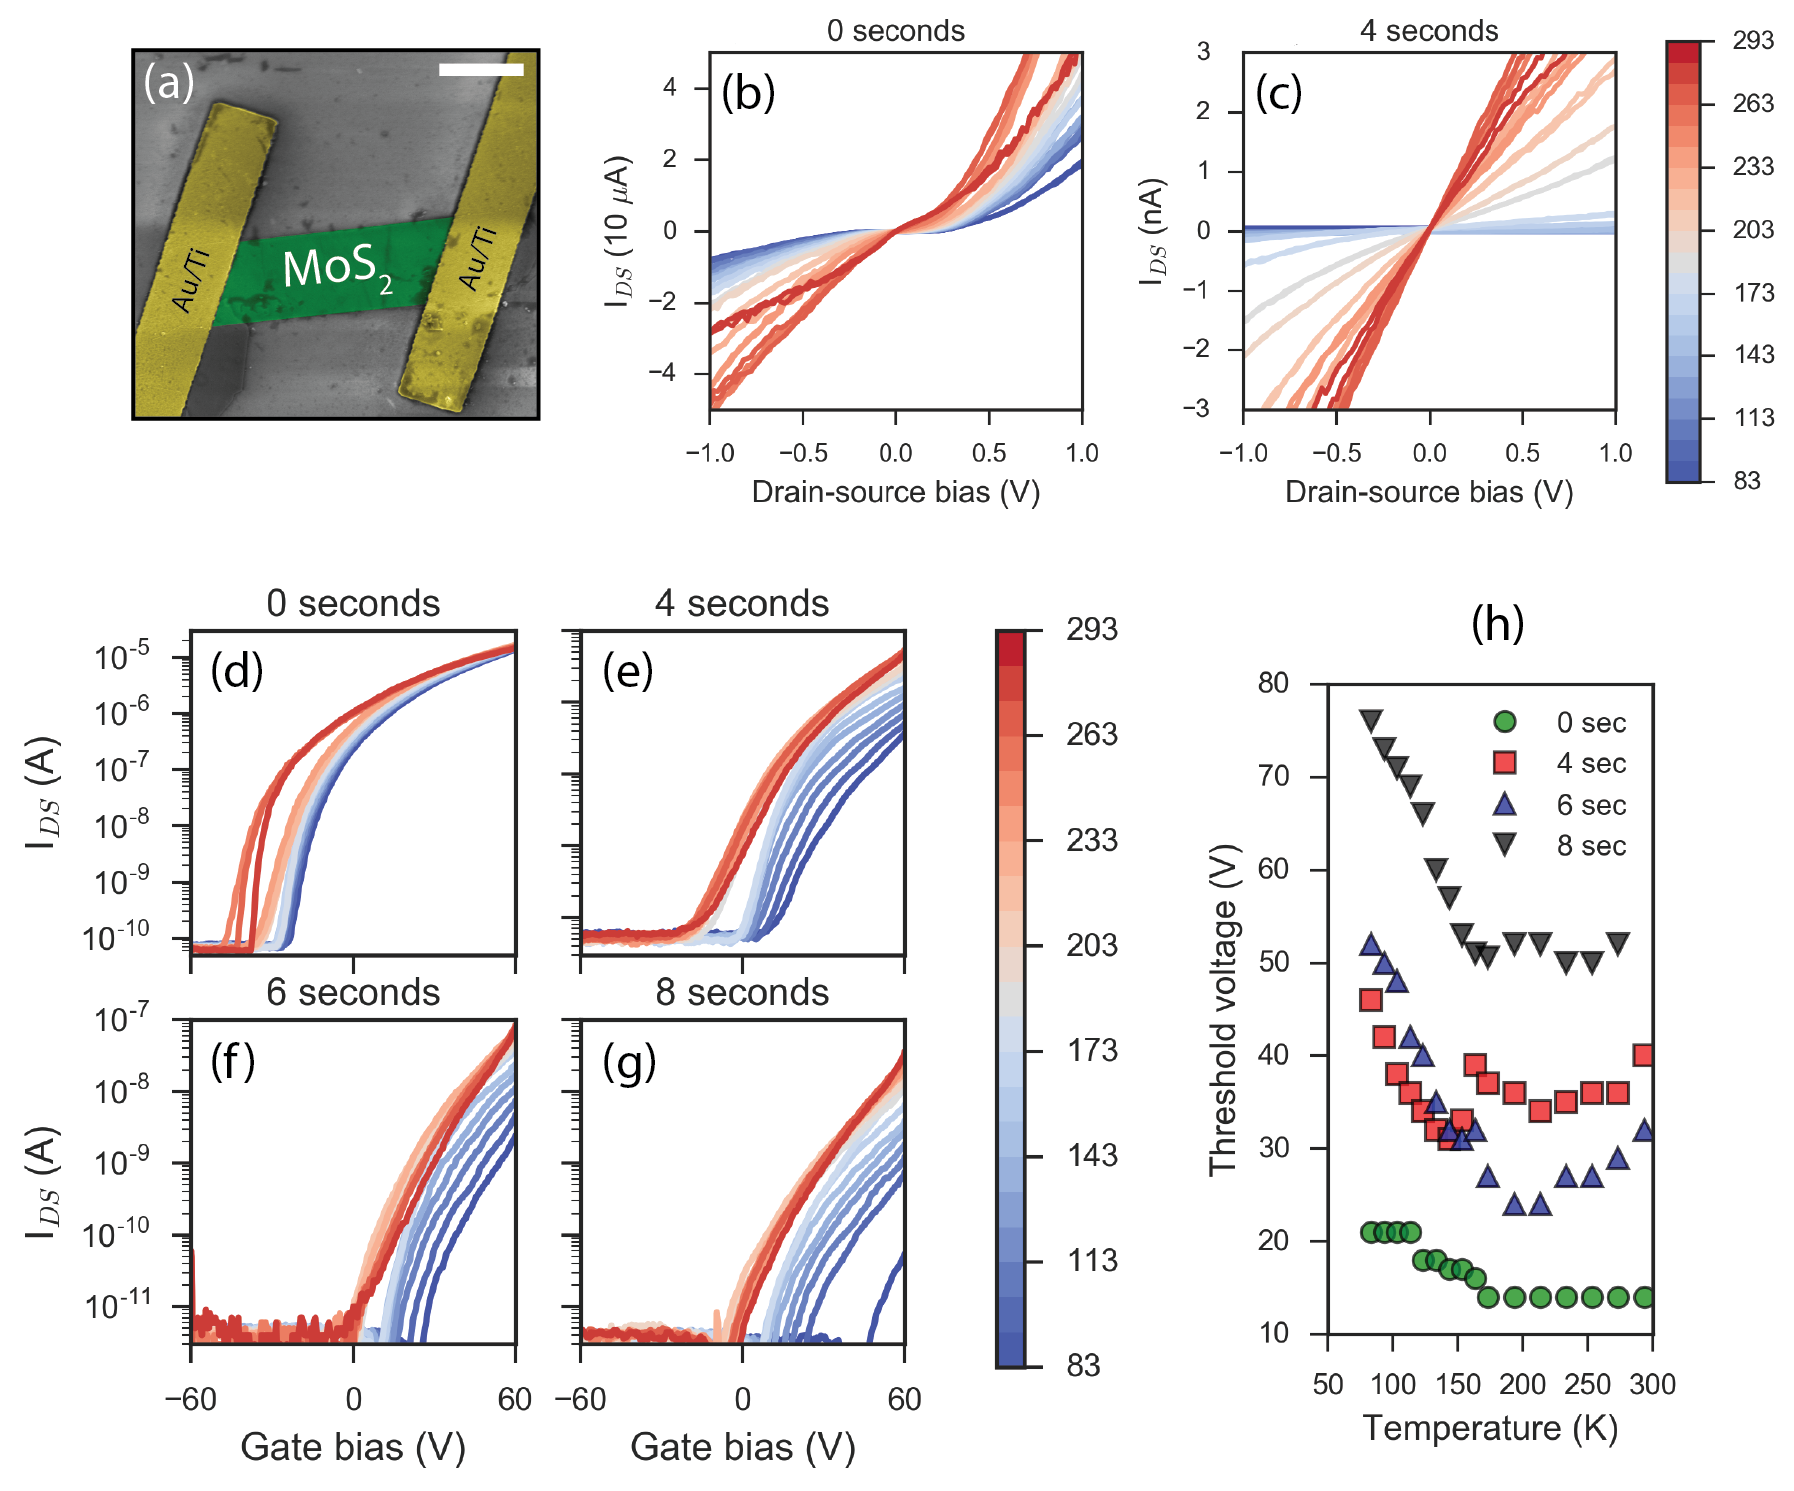
\includegraphics[width=\columnwidth]{Figs_1.png}
\caption{{\footnotesize \textbf{Characterisation of MoS$_2$ FET devices: (a) False color SEM image of a typical bilayer MoS$_2$ device. The scale bar is 1 $\mu$m. (b)-(c) IV characteristics of the device before and after 4 seconds of plasma treatment. The curves are color-mapped to the measurement temperatures indicate on the color bar on the right. (d)-(g) Gate characteristics of the same device, after each subsequent plasma exposure. The colors correspond to temperatures in Kelvin on the color bar on the right. (h) Plot indicating the shift in threshold voltage of the FET with temperature for the different exposure times. }}}
\label{fig:electrical}
\end{figure}}
After each exposure, they were removed and characterised electrically in a two-probe configuration in an \textit{in-situ} cryogenic stage environment (NAME OF CRYO STAGE COMPANY), cooled by liquid N$_2$, inside a SEM chamber maintained at a pressure of $10^{-4}$ mbar. Tungsten nanomanipulator tips (Imina miBot) served as source and drain terminals powered by an Agilent B2912A dual channel sourcemeter. The measurements were taken starting at the lowest temperature and finishing at room temperature. Before each characterisation at a new temperature, the system was left to equilibrate so that the temperature did not vary by more than 1 K for longer than 5 minutes. The samples were then removed from the system and exposed to the ambient when transferring to the plasma cleaner for further plasma treatment. The whole experiment was performed within 1 day to avoid storing the sample for a long time. \newline
\indent The IV curves measured at zero gate bias shown in \textbf{Fig. 1(b)-(c)} demonstrate the effect of plasma treatment on the transport properties of the MoS$_2$ sample. Before treatment, the device outputs tens of microamps at drain-source bias of V$_{ds}$ = $\pm 1$ V even at cryogenic temperatures. The semiconducting nature of the material is evident from the transport gap observed around the zero-point at low temperatures, and the non-linearity of the sweeps. After 4 seconds of plasma treatment, however, the output characteristics change to a more Ohmic nature, with a clear linear relationship emerging between the applied bias and the output current I$_{ds}$. Importantly, the produced current has now dropped several orders of magnitude, with the device now only outputting several nanoamps at the same V$_{ds}$ as before plasma exposure. Subsequent treatments to 6 and 8 seconds drop the current levels to the noise floor of the instrument (see Supporting Information). \newline
\indent The transfer characteristics of the same device were also tested at different temperatures and are presented in \textbf{Fig. 1(d)-(g)}. The 0 second gate sweeps follow standard literature observations, with onset in the negative gate bias region, and a temperature dependence for the sweeps first noted by Jariwala et al \cite{jariwala2013band}. Further measurements after plasma exposures yield a different behaviour for the device. The current magnitude drops significantly as exposure time increases, while the threshold voltage, V$_{th}$, is seen to drastically shift to large positive gate biases with decreasing temperature. This dependence is charted in \textbf{Fig. 1(h)} for all exposure times, indicating an almost linear increase in V$_{th}$ past a certain temperature after each exposure time; an approximation often utilised for MOSFETs \cite{filanovsky2001mutual}. \newline
\indent Around 200K a clear gap, $\Delta$V$_{th}$, develops in the gate sweeps, separating the blue curves from the red ones along the gate bias axis. At the same time, the treated devices are seen to deviate from standard MoS$_2$ FET characteristics. The subthreshold and linear regions of the transistor cannot now be easily distinguished, while the ramp up to saturation adopts a constrained shape, especially at low temperatures, with none of the devices reaching the saturation region completely due to the large V$_{th}$ shift. As this is also seen in the pristine sample, we do not attribute the origin of this $\Delta$V$_{th}$ to the plasma treatment process, though it necessitates further investigation in the future.




{\setlength\intextsep{5pt}
\begin{figure}
\centering
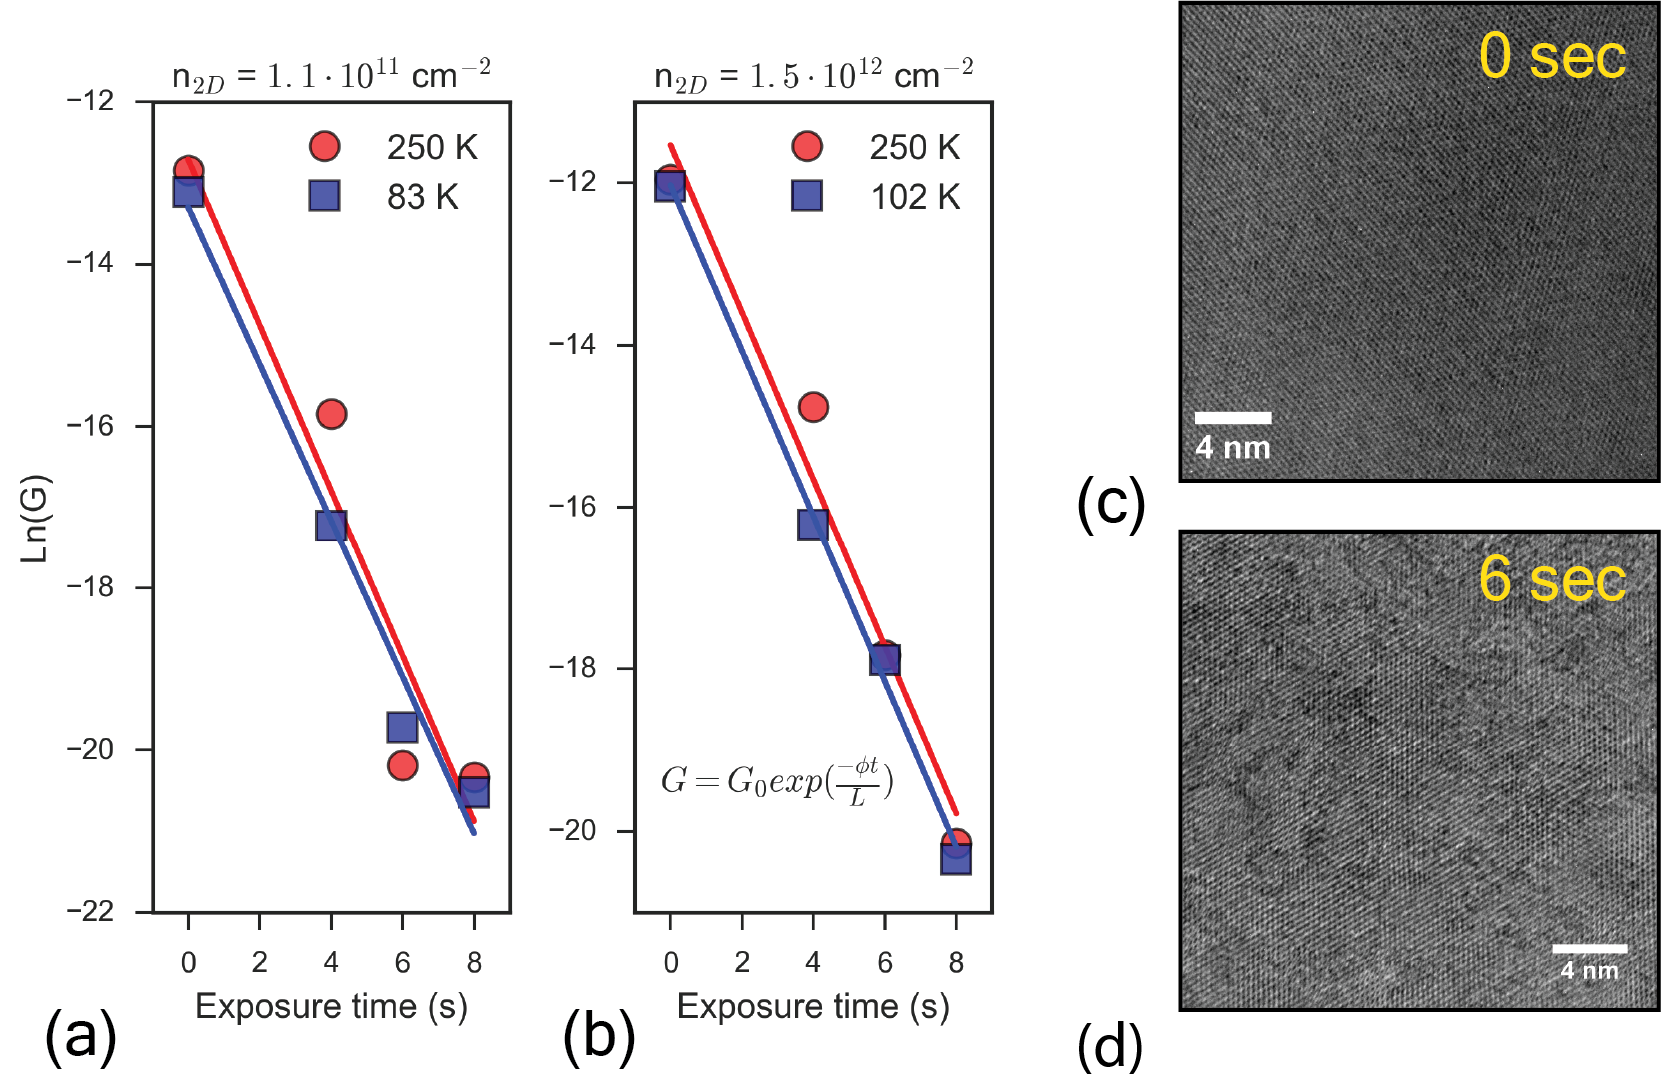
\includegraphics[width=\columnwidth]{Figs_2.png}
\caption{{\footnotesize \textbf{Effect of plasma treatment on device conductance, $G$: (a) Arrhenius plot of $G$ after different exposure times for the same device at a carrier density of $n_{2D}$ = $1.5\cdot 10^{11}$ $cm^{-2}$. (b) Activation energies, $E_A$, extracted from the linear fits in (a), showing variation with plasma exposure time. (c) Log-log plot of device field effect mobility as a function of temperature after 4 seconds of plasma treatement. (d)-(e) Semi-log plots demonstrating the exponential decay of conductance with plasma time at carrier densities of $n_{2D}$ = $1.5\cdot 10^{11}$ $cm^{-2}$ and $n_{2D}$ = $1.5\cdot 10^{12}$ $cm^{-2}$ respectively. }}}
\label{fig:electrical}
\end{figure}}
The thermally-activated conductance characteristics of the MoS$_2$ FET are studied after different exposure times in \textbf{Fig. 2(a)}. A notable drop in conductance at all temperatures is observed after plasma treatment is initiated. In addition, the low temperature regime shows a significant further drop in conductance, indicating a possible additional contribution to scattering from plasma-created defects in the MoS$_2$. From the linear Arrhenius fits to the data in (a), we extract the activation energy for thermal transport at each of the exposure times and chart them in \textbf{Fig. 2(b)}. We note a large increase in $E_A$ after 4 seconds of exposure at the same back-gate voltage, signifying an inhibited ability of carriers to be promoted to the conduction band in this newly-created defective system, which is confirmed by the threshold voltage shift discussed previously. The activated transport property which now emerges strongly in the device \newline
\indent Similarly, the mobility is tracked as a function of temperature on the log-log plot in \textbf{Fig. 2(c)}. We see that a drastic drop in mobility occurs past a temperature of about 170K. From Mathiessen's rule, it is known that the residual resistivity at low temperatures is due to the impurity scattering term, $\mu_{imp}^{-1}$, which comprises both the long range and short range Coulombic scattering components \cite{cui2015multi}. In encapsulated and pristine MoS$_2$ FETs, this has been shown to dominate transport properties below 100K \cite{radisavljevic2013mobility, cui2015multi}. In the presently discussed case of plasma-modified MoS$_2$, the impurity concentration is high enough to allow for dominant impurity contribution at much higher temperatures of $\sim$170K. The increased role of scattering in the low temperature regime for the treated device may come from the increased interfacial scattering term due to the inevitable presence of molybdenum oxides on the surface of the device, as well as sulfur vacancies originating from plasma-etched regions \cite{ko2016stack, zhu2016remote, jadwiszczak2017oxide}. Although $\mu_{imp}$ is independent of $T$, it does increase with $n_{2D}$ which is expected to change with the degree of surface-bound oxides which are present on the surface. \newline
\indent In addition, we track the conductance drop in the sample with increasing plasma exposure time at different carrier densities and in the high and low temperature regimes in \textbf{Fig. (d)-(e)}. From the semi-logarithmic plots, we find good fits confirming an exponential drop in conductance. The layer number-normalised exponential drop in mobility over time in oxygen plasma-treated MoS$_2$ has been previously been reported \cite{khondaker2016bandgap} as: 
\begin{equation}
\mu L^{-1} (t) \approx exp(- \phi t/L) 
\end{equation} where $L$ is the layer number, $\phi = \dot{\mu}/\mu$ and $\dot{\mu}$ is the time derivative of the mobility. Following this convention, we can extract the time rate of change of the conductance in our bilayer sample, with $\phi_{G} = \dot{G}/G$ = 2.02/s. The contribution of MoO$_3$ species formed by the oxygen-containing plasma may lead to the formation of an effective semiconducting medium in the FET channel, giving rise to the exponential dependence of current tunnelling at the newly formed heterostructure-like interface \cite{khondaker2016bandgap, choudhary2016two}.



{\setlength\intextsep{5pt}
\begin{figure}
\centering
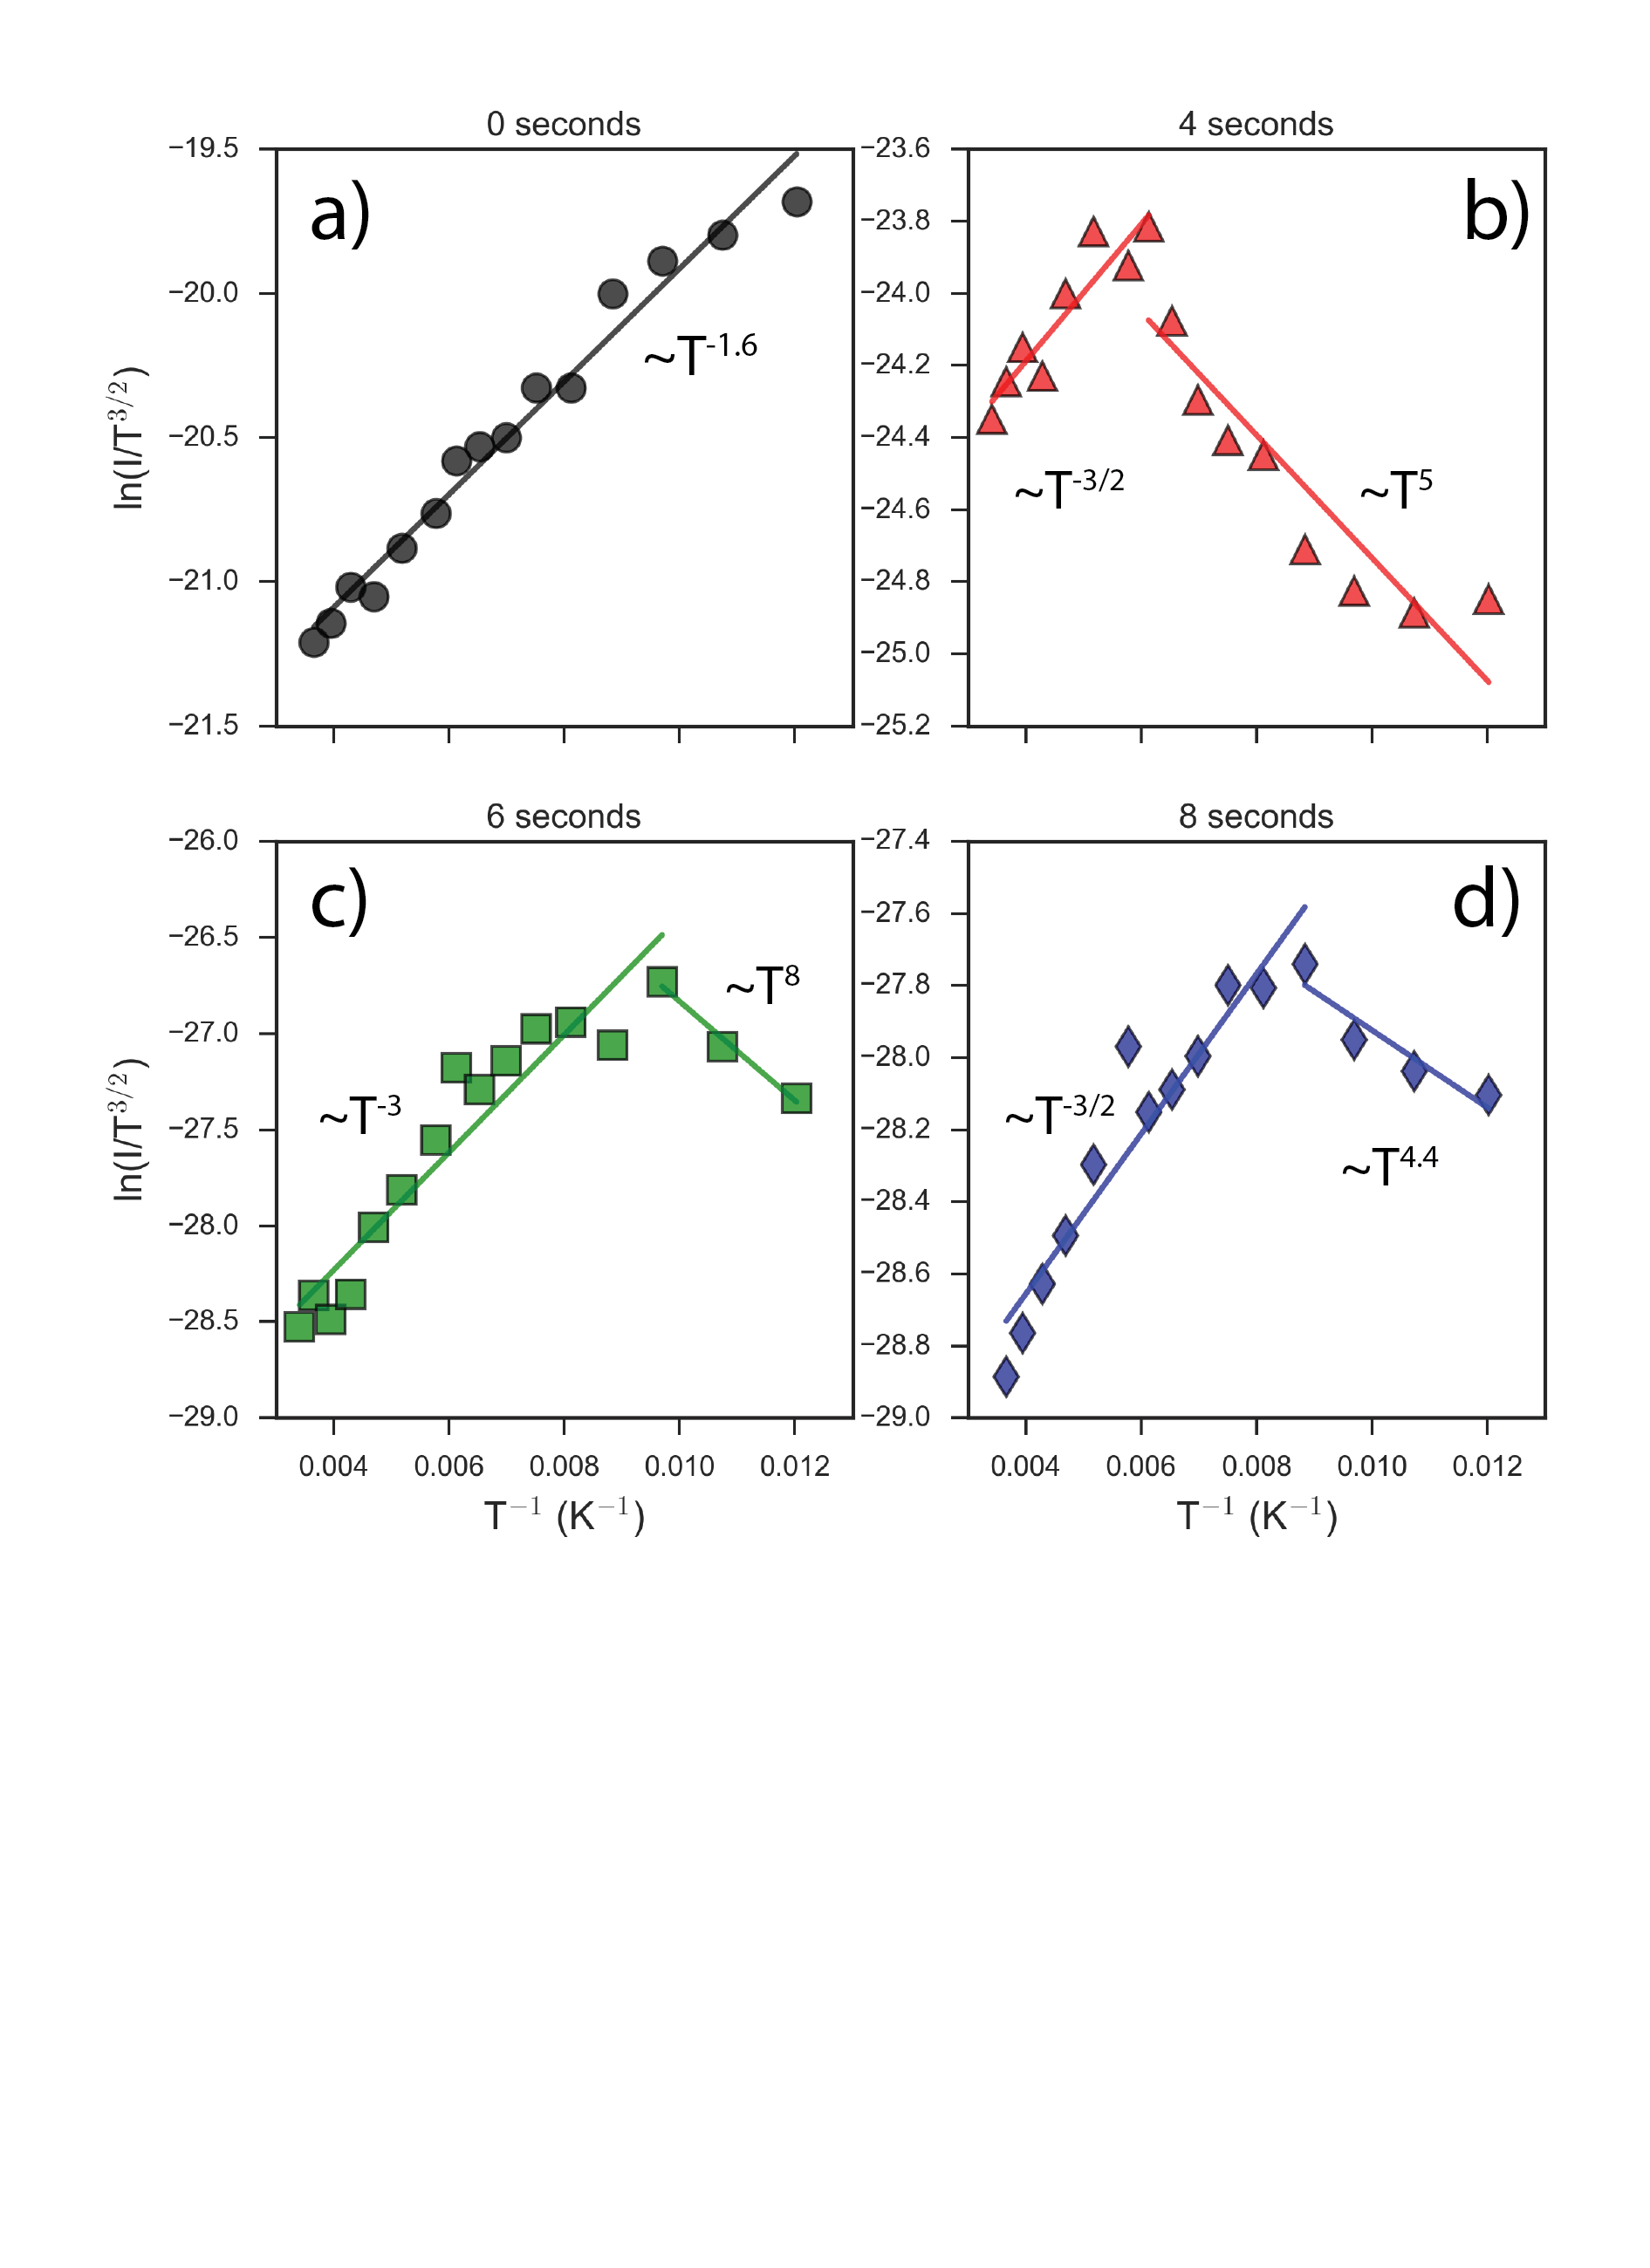
\includegraphics[width=\columnwidth]{Figure_4.png}
\caption{{\footnotesize \textbf{Richardson plots at different plasma treatment times: (a) Standard Richardson plot for a pristne 2D MoS$_2$ FET exemplifying a consistent relationship of the current to applied temperature across the range 83-293K. (b) Upon plasma treatment, the current emission mechanism changes abruptly once the device is cooled down. Two distinct regimes emerge which can both be fitted with a power law. Similar scaling is observed in the 6 and 8 second plots in (c) and (d), although less current is outputted by the device, consistent with the conductance drop observed in \textbf{Fig. 2}.  }}}
\label{fig:electrical}
\end{figure}}

{\setlength\intextsep{5pt}
\begin{figure}
\centering
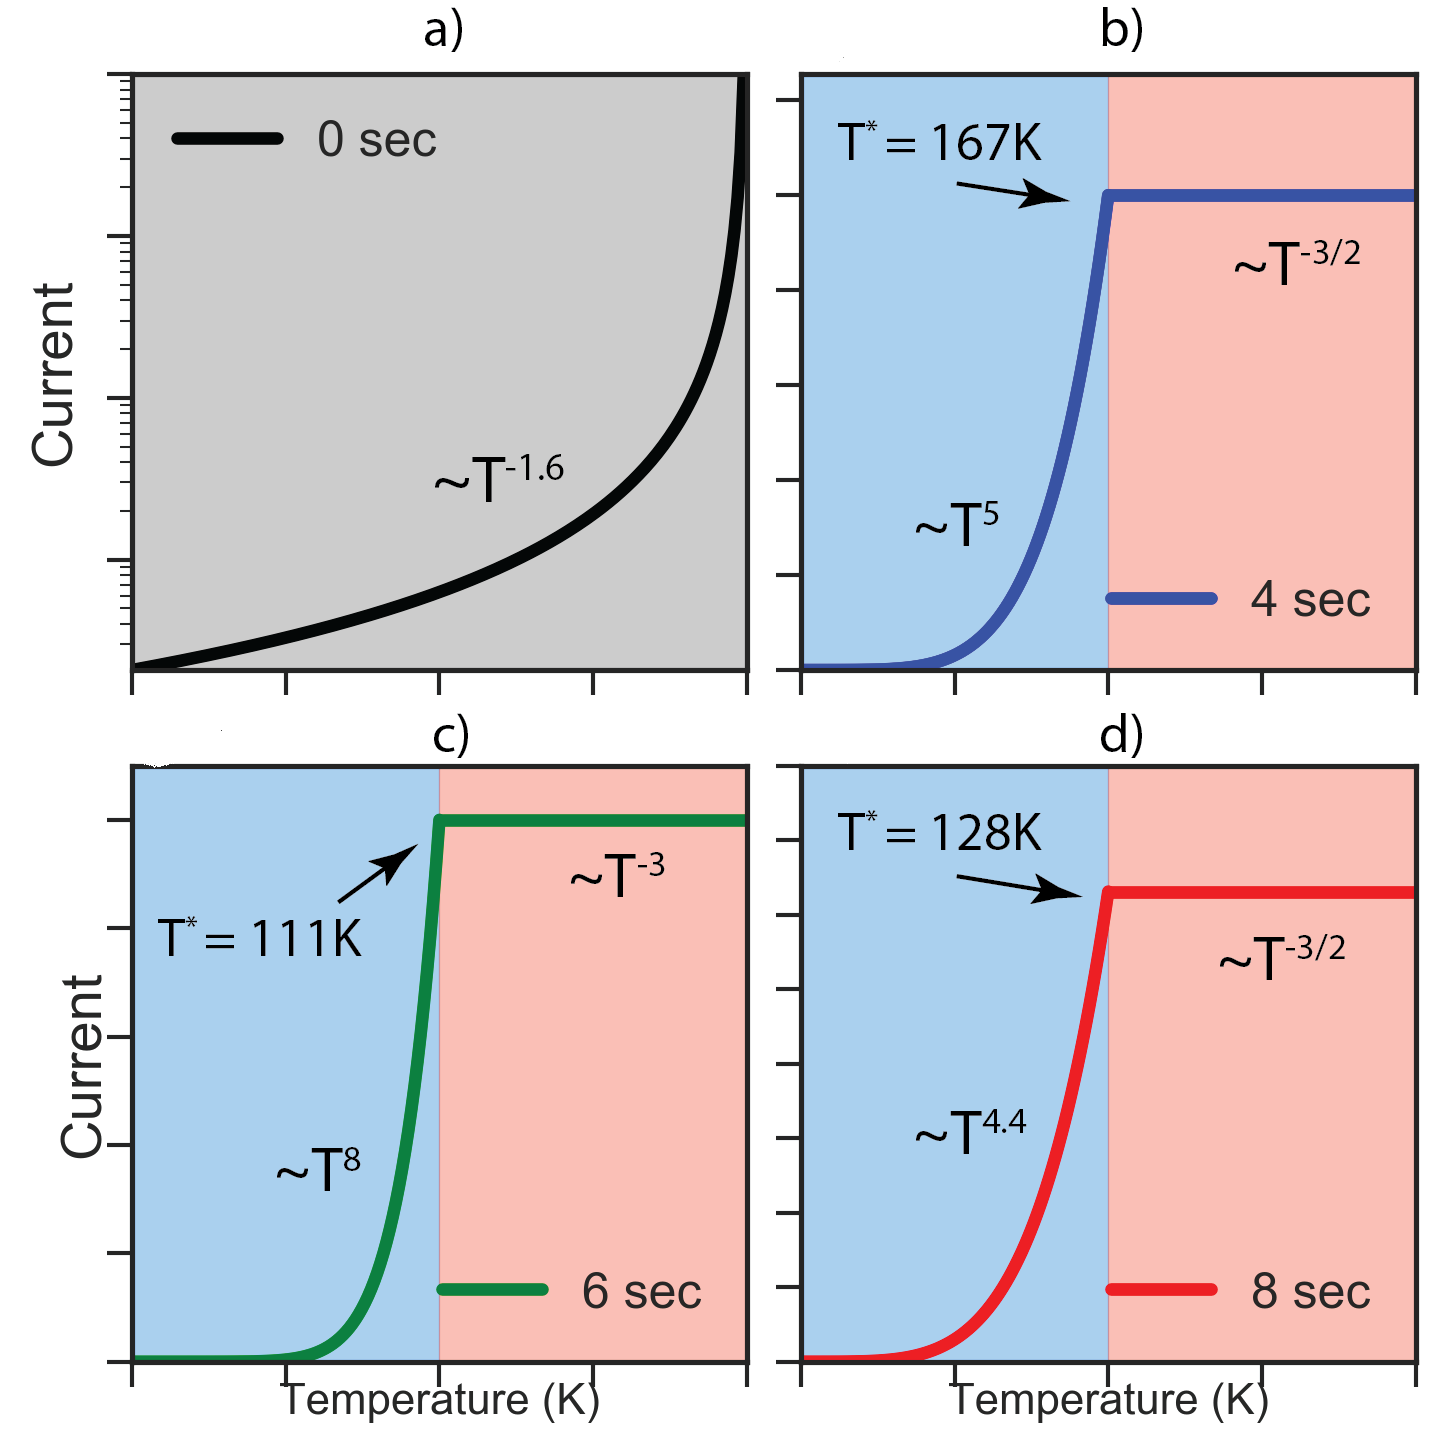
\includegraphics[width=\columnwidth]{Fig_5.png}
\caption{{\footnotesize \textbf{CAPTION CAPTION CAPTION}}}
\label{fig:electrical}
\end{figure}}

\indent Charge injection from the electrode into the 2D semiconductor (at moderate doping levels) is mostly governed by thermionic emission over the Schottky barrier and the persistent van der Waals gap which exists at the interface \cite{allain2015electrical}. Furthermore, Fermi level pinning occurs near the bottom of the conduction band of the MoS$_2$, independent of metal work function \cite{kim2017fermi}. When considering current injection for a 2D system, one needs to account for confinement effects \cite{anwar1999effects}, hence the Richardson equation is modified as follows:
\begin{equation}
\displaystyle I_{2D} = AA^{*}_{2D} T^{3/2} exp\left( \frac{-q \phi_B}{k_B T} \right) exp\left( \frac{q V_{DS}}{k_B T} \right)
\end{equation}where $A$ is the junction area, $A^{*}_{2D}$ is the Richardson constant for a 2D system, $T$ is temperature, $q$ the Coulombic charge, $k_B$ is the Boltzmann constant, $\phi_B$ is the effective Schottky barrier height and $V_{DS}$ is the drain-source bias. We note that $I$ scales as $T^{3/2}$ for a 2D system such as the MoS$_2$ FET \cite{wang2016high,kim2017fermi,somvanshi2017nature}, and $\phi_B$ can thus be extracted from the slope of the $ln(IT^{-3/2})$ vs $T^{-1}$ curve.

\clearpage 

\bibliographystyle{apsrev}

\bibliography{lowT}

\end{document}
%
% ****** End of file aipsamp.tex ******
